% Options for packages loaded elsewhere
\PassOptionsToPackage{unicode}{hyperref}
\PassOptionsToPackage{hyphens}{url}
%
\documentclass[
]{article}
\usepackage{amsmath,amssymb}
\usepackage{iftex}
\ifPDFTeX
  \usepackage[T1]{fontenc}
  \usepackage[utf8]{inputenc}
  \usepackage{textcomp} % provide euro and other symbols
\else % if luatex or xetex
  \usepackage{unicode-math} % this also loads fontspec
  \defaultfontfeatures{Scale=MatchLowercase}
  \defaultfontfeatures[\rmfamily]{Ligatures=TeX,Scale=1}
\fi
\usepackage{lmodern}
\ifPDFTeX\else
  % xetex/luatex font selection
\fi
% Use upquote if available, for straight quotes in verbatim environments
\IfFileExists{upquote.sty}{\usepackage{upquote}}{}
\IfFileExists{microtype.sty}{% use microtype if available
  \usepackage[]{microtype}
  \UseMicrotypeSet[protrusion]{basicmath} % disable protrusion for tt fonts
}{}
\makeatletter
\@ifundefined{KOMAClassName}{% if non-KOMA class
  \IfFileExists{parskip.sty}{%
    \usepackage{parskip}
  }{% else
    \setlength{\parindent}{0pt}
    \setlength{\parskip}{6pt plus 2pt minus 1pt}}
}{% if KOMA class
  \KOMAoptions{parskip=half}}
\makeatother
\usepackage{xcolor}
\usepackage[margin=1in]{geometry}
\usepackage{color}
\usepackage{fancyvrb}
\newcommand{\VerbBar}{|}
\newcommand{\VERB}{\Verb[commandchars=\\\{\}]}
\DefineVerbatimEnvironment{Highlighting}{Verbatim}{commandchars=\\\{\}}
% Add ',fontsize=\small' for more characters per line
\usepackage{framed}
\definecolor{shadecolor}{RGB}{248,248,248}
\newenvironment{Shaded}{\begin{snugshade}}{\end{snugshade}}
\newcommand{\AlertTok}[1]{\textcolor[rgb]{0.94,0.16,0.16}{#1}}
\newcommand{\AnnotationTok}[1]{\textcolor[rgb]{0.56,0.35,0.01}{\textbf{\textit{#1}}}}
\newcommand{\AttributeTok}[1]{\textcolor[rgb]{0.13,0.29,0.53}{#1}}
\newcommand{\BaseNTok}[1]{\textcolor[rgb]{0.00,0.00,0.81}{#1}}
\newcommand{\BuiltInTok}[1]{#1}
\newcommand{\CharTok}[1]{\textcolor[rgb]{0.31,0.60,0.02}{#1}}
\newcommand{\CommentTok}[1]{\textcolor[rgb]{0.56,0.35,0.01}{\textit{#1}}}
\newcommand{\CommentVarTok}[1]{\textcolor[rgb]{0.56,0.35,0.01}{\textbf{\textit{#1}}}}
\newcommand{\ConstantTok}[1]{\textcolor[rgb]{0.56,0.35,0.01}{#1}}
\newcommand{\ControlFlowTok}[1]{\textcolor[rgb]{0.13,0.29,0.53}{\textbf{#1}}}
\newcommand{\DataTypeTok}[1]{\textcolor[rgb]{0.13,0.29,0.53}{#1}}
\newcommand{\DecValTok}[1]{\textcolor[rgb]{0.00,0.00,0.81}{#1}}
\newcommand{\DocumentationTok}[1]{\textcolor[rgb]{0.56,0.35,0.01}{\textbf{\textit{#1}}}}
\newcommand{\ErrorTok}[1]{\textcolor[rgb]{0.64,0.00,0.00}{\textbf{#1}}}
\newcommand{\ExtensionTok}[1]{#1}
\newcommand{\FloatTok}[1]{\textcolor[rgb]{0.00,0.00,0.81}{#1}}
\newcommand{\FunctionTok}[1]{\textcolor[rgb]{0.13,0.29,0.53}{\textbf{#1}}}
\newcommand{\ImportTok}[1]{#1}
\newcommand{\InformationTok}[1]{\textcolor[rgb]{0.56,0.35,0.01}{\textbf{\textit{#1}}}}
\newcommand{\KeywordTok}[1]{\textcolor[rgb]{0.13,0.29,0.53}{\textbf{#1}}}
\newcommand{\NormalTok}[1]{#1}
\newcommand{\OperatorTok}[1]{\textcolor[rgb]{0.81,0.36,0.00}{\textbf{#1}}}
\newcommand{\OtherTok}[1]{\textcolor[rgb]{0.56,0.35,0.01}{#1}}
\newcommand{\PreprocessorTok}[1]{\textcolor[rgb]{0.56,0.35,0.01}{\textit{#1}}}
\newcommand{\RegionMarkerTok}[1]{#1}
\newcommand{\SpecialCharTok}[1]{\textcolor[rgb]{0.81,0.36,0.00}{\textbf{#1}}}
\newcommand{\SpecialStringTok}[1]{\textcolor[rgb]{0.31,0.60,0.02}{#1}}
\newcommand{\StringTok}[1]{\textcolor[rgb]{0.31,0.60,0.02}{#1}}
\newcommand{\VariableTok}[1]{\textcolor[rgb]{0.00,0.00,0.00}{#1}}
\newcommand{\VerbatimStringTok}[1]{\textcolor[rgb]{0.31,0.60,0.02}{#1}}
\newcommand{\WarningTok}[1]{\textcolor[rgb]{0.56,0.35,0.01}{\textbf{\textit{#1}}}}
\usepackage{graphicx}
\makeatletter
\def\maxwidth{\ifdim\Gin@nat@width>\linewidth\linewidth\else\Gin@nat@width\fi}
\def\maxheight{\ifdim\Gin@nat@height>\textheight\textheight\else\Gin@nat@height\fi}
\makeatother
% Scale images if necessary, so that they will not overflow the page
% margins by default, and it is still possible to overwrite the defaults
% using explicit options in \includegraphics[width, height, ...]{}
\setkeys{Gin}{width=\maxwidth,height=\maxheight,keepaspectratio}
% Set default figure placement to htbp
\makeatletter
\def\fps@figure{htbp}
\makeatother
\setlength{\emergencystretch}{3em} % prevent overfull lines
\providecommand{\tightlist}{%
  \setlength{\itemsep}{0pt}\setlength{\parskip}{0pt}}
\setcounter{secnumdepth}{-\maxdimen} % remove section numbering
\ifLuaTeX
  \usepackage{selnolig}  % disable illegal ligatures
\fi
\IfFileExists{bookmark.sty}{\usepackage{bookmark}}{\usepackage{hyperref}}
\IfFileExists{xurl.sty}{\usepackage{xurl}}{} % add URL line breaks if available
\urlstyle{same}
\hypersetup{
  pdftitle={Coding Assignment 1},
  pdfauthor={Team N},
  hidelinks,
  pdfcreator={LaTeX via pandoc}}

\title{Coding Assignment 1}
\author{Team N}
\date{Due: 2023-10-01 23:59}

\begin{document}
\maketitle

{
\setcounter{tocdepth}{2}
\tableofcontents
}
\begin{Shaded}
\begin{Highlighting}[]
\CommentTok{\# Put any packages you want here}
\end{Highlighting}
\end{Shaded}

A Florida health insurance company wants to predict annual claims for
individual clients. The company pulls a random sample of 100 customers.
The owner wishes to charge an actuarially fair premium to ensure a
normal rate of return. The owner collects all of their current
customer's health care expenses from the last year and compares them
with what is known about each customer's plan.

The data on the 100 customers in the sample is as follows:

\begin{itemize}
\tightlist
\item
  Charges: Total medical expenses for a particular insurance plan (in
  dollars)
\item
  Age: Age of the primary beneficiary
\item
  BMI: Primary beneficiary's body mass index (kg/m2)
\item
  Female: Primary beneficiary's birth sex (0 = Male, 1 = Female)
\item
  Children: Number of children covered by health insurance plan
  (includes other dependents as well)
\item
  Smoker: Indicator if primary beneficiary is a smoker (0 = non-smoker,
  1 = smoker)
\item
  Cities: Dummy variables for each city with the default being Sanford
\end{itemize}

Answer the following questions using complete sentences and attach all
output, plots, etc. within this report.

\textbf{For this assignment, ignore the categorical variables (gender,
smoker, cities)}

\hypertarget{question-1}{%
\section{Question 1}\label{question-1}}

Perform univariate analyses on the quantitative variables (center,
shape, spread). Include descriptive statistics, and histograms. Be sure
to use terms discussed in class such as bimodal, skewed left, etc.

\begin{Shaded}
\begin{Highlighting}[]
\FunctionTok{summary}\NormalTok{(Insurance\_Data\_Group15}\SpecialCharTok{$}\NormalTok{Charges)}
\end{Highlighting}
\end{Shaded}

\begin{verbatim}
##    Min. 1st Qu.  Median    Mean 3rd Qu.    Max. 
##    1534    4788    8680   12381   13884   62593
\end{verbatim}

\begin{Shaded}
\begin{Highlighting}[]
\FunctionTok{hist}\NormalTok{(Insurance\_Data\_Group15}\SpecialCharTok{$}\NormalTok{Charges)}
\end{Highlighting}
\end{Shaded}

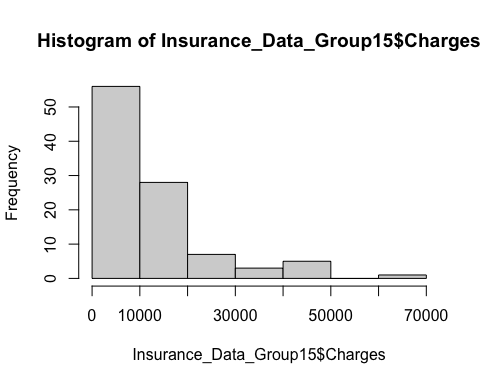
\includegraphics{CodingAssignment01_files/figure-latex/q1-1.pdf}

\begin{Shaded}
\begin{Highlighting}[]
\FunctionTok{summary}\NormalTok{(Insurance\_Data\_Group15}\SpecialCharTok{$}\NormalTok{Age)}
\end{Highlighting}
\end{Shaded}

\begin{verbatim}
##    Min. 1st Qu.  Median    Mean 3rd Qu.    Max. 
##   18.00   27.00   38.50   39.28   52.25   64.00
\end{verbatim}

\begin{Shaded}
\begin{Highlighting}[]
\FunctionTok{hist}\NormalTok{(Insurance\_Data\_Group15}\SpecialCharTok{$}\NormalTok{Age)}
\end{Highlighting}
\end{Shaded}

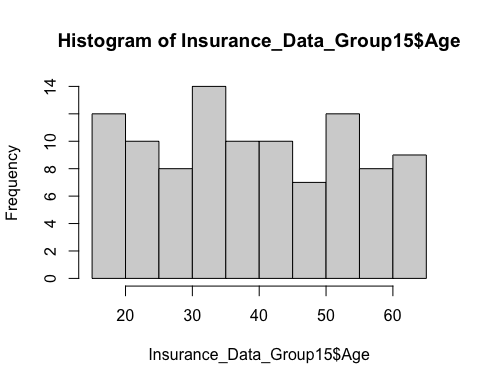
\includegraphics{CodingAssignment01_files/figure-latex/q1-2.pdf}

\begin{Shaded}
\begin{Highlighting}[]
\FunctionTok{summary}\NormalTok{(Insurance\_Data\_Group15}\SpecialCharTok{$}\NormalTok{BMI)}
\end{Highlighting}
\end{Shaded}

\begin{verbatim}
##    Min. 1st Qu.  Median    Mean 3rd Qu.    Max. 
##   17.40   25.20   30.43   30.03   34.47   46.75
\end{verbatim}

\begin{Shaded}
\begin{Highlighting}[]
\FunctionTok{hist}\NormalTok{(Insurance\_Data\_Group15}\SpecialCharTok{$}\NormalTok{BMI)}
\end{Highlighting}
\end{Shaded}

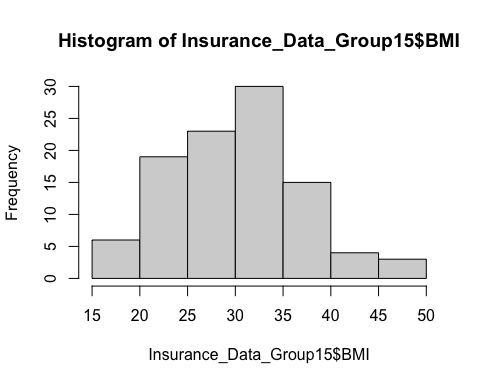
\includegraphics{CodingAssignment01_files/figure-latex/q1-3.pdf}

\begin{Shaded}
\begin{Highlighting}[]
\FunctionTok{summary}\NormalTok{(Insurance\_Data\_Group15}\SpecialCharTok{$}\NormalTok{Children)}
\end{Highlighting}
\end{Shaded}

\begin{verbatim}
##    Min. 1st Qu.  Median    Mean 3rd Qu.    Max. 
##     0.0     0.0     1.0     1.2     2.0     5.0
\end{verbatim}

\begin{Shaded}
\begin{Highlighting}[]
\FunctionTok{hist}\NormalTok{(Insurance\_Data\_Group15}\SpecialCharTok{$}\NormalTok{Children)}
\end{Highlighting}
\end{Shaded}

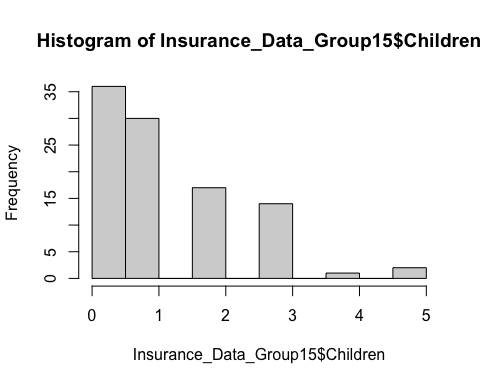
\includegraphics{CodingAssignment01_files/figure-latex/q1-4.pdf} room
for description

\hypertarget{question-2}{%
\section{Question 2}\label{question-2}}

Perform bivariate analyses on the quantitative variables (direction,
strength and form). Describe the linear association between all
variables.

\begin{Shaded}
\begin{Highlighting}[]
\FunctionTok{plot}\NormalTok{(Insurance\_Data\_Group15}\SpecialCharTok{$}\NormalTok{Age, Insurance\_Data\_Group15}\SpecialCharTok{$}\NormalTok{Charges)}
\end{Highlighting}
\end{Shaded}

\includegraphics{CodingAssignment01_files/figure-latex/q2-1.pdf}

\begin{Shaded}
\begin{Highlighting}[]
\CommentTok{\# Question 3}
\end{Highlighting}
\end{Shaded}

also write out the regression cleanly in this document.

\hypertarget{question-4}{%
\section{Question 4}\label{question-4}}

An eager insurance representative comes back with a potential client.
The client is 40, their BMI is 30, and they have one dependent. Using
the regression equation above, predict the amount of medical expenses
associated with this policy. (Provide a 95\% confidence interval as
well)

\end{document}
